%!TEX root = ../Thesis.tex

\section{Paragraph2vec}

The Skip-gram model only directly allows to get a vector representation of a single word, not a sentence or more. However to find a vector representation for a news article one must work on a sentence level. A simple approach is to just take the avenge vector sum of all the words in the article title and perhaps the subhead.

While this method is perfectly valid it neglects the order of words just like the bag-of-word methods. As a solution to this the paragraph2vec model has been sugested. This is a set of models that looks very similar to the skip-gram model (or word2vec in general), but also learns a document vector which can be learned to capture the content of a document.

The model shown here is the Distributed Memory Model of Paragraph Vectors (short PV-DM), as it has been shown to provide the best results \cite{doc2vec}. 

\subsection{Forward-pass}

The idea behind the PV-DM model is a bit different from the skip-gram model. Instead of using one word to predict multiply surrounding words, it uses a window of previous words to predict just a single word. In addition to this, the model uses a unique document vector for each document to adjust the word probabilities.

\begin{figure}[H]
	\centering
	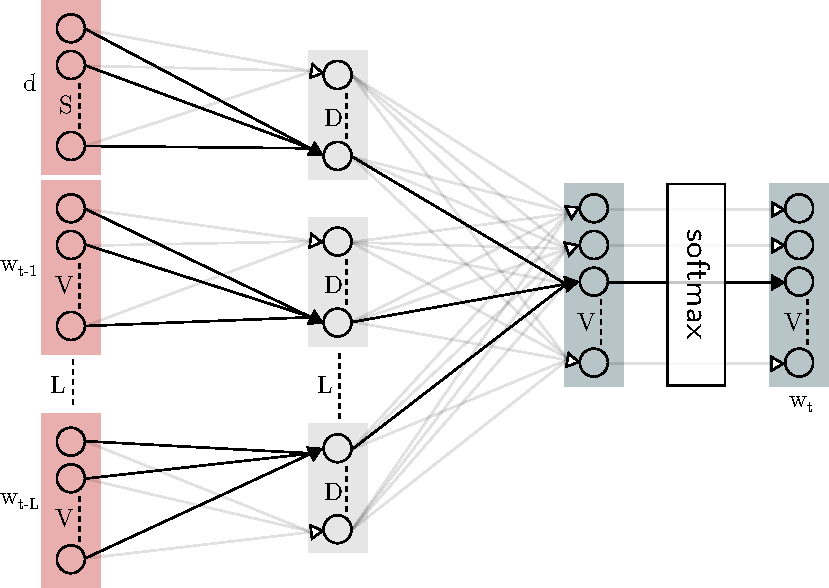
\includegraphics[scale=0.7]{theory/doc2vec-network}
	\caption{Visualization of the paragraph2vec model called ``Distributed Memory Model of Paragraph Vectors''.}
	\label{fig:theory:doc2vec:network}
\end{figure}

Lets denote the indicator vector for the word at position $t$ in a document as $\{x_i^{w_t}\}_{i=1}^V$. The indicator vector describing the document $d$ is then $\{x_i^d\}_{i=1}^S$, where $S$ is the amount of documents. The document vectors $b_{h_1}^d$ and word vectors are then calculated as:
\begin{equation}
\begin{aligned}
b_{h_1}^{w_{t-\ell}} &= a_{h_1}^{w_{t-\ell}} = \sum_{i=1}^V w_{i,h_1} x_{i}^{w_{t-\ell}} && \forall \ell \in [1, L], h_1 \in [1, D] \\
b_{h_1}^d &= a_{h_1}^d = \sum_{i=1}^S d_{i,h_1} x_{i}^d && \forall h_1 \in [1, D]
\end{aligned}
\end{equation}

Note that the document vector is unique for each document but shared for all word prediction in that document. The word vectors are then shared across all documents, just like in the skip-gram model.

The document and word vectors are then concatenated intro a single vector, which is then multiplied by a weight matrix to generate the softmax input for the word prediction.
\begin{equation}
\begin{aligned}
a_{k}^t &= a_{h_2}^t = \sum_{\ell=1}^L \sum_{h_1}^D w_{h_1 + \ell \cdot D, h_2} b_{h_1}^{w_{t - \ell}} + \sum_{h_1}^D w_{h_1, h_2} b_{h_1}^d && \forall k \in [1, V] \\
y_{k}^t &= \frac{\exp(a_k^t)}{\sum_{k'=1}^V \exp(a_{k'}^t)} && \forall k \in [1, V]
\end{aligned}
\end{equation}

The softmax used to calculate $y_{k}^t$ performs a very large sum. This sum is impractical to calculate, for this reason the paper \cite{doc2vec} suggest using an approximation called hierarchical softmax.

The model is trained just like the skip-gram model, that is using stochastic gradient decent. This optimizes the document and word vectors jointly. It is possible to later fix the word vectors and only train the document vector, but that wasn't done in this case.
